\section{Medição e Análise: GQM}

O método GQM foi originalmente desenvolvido por V. Basili e D. Weiss e expandido com muitos outros conceitos por D.  Rombach. O GQM apóia muito bem a abordagem de melhoria da qualidade orientada aos negócios e resulta de muitos anos de experiência prática e pesquisa acadêmica \cite{solingen}.

A qualidade é um aspecto importante para atrair clientes e muitas abordagens estão disponíveis para melhorar os processos de software a fim de resolver problemas que ocorrem durante o desenvolvimento do mesmo, por exemplo, os projetos são concluídos muito tarde, excedem seus orçamentos ou exigem substancialmente mais recursos do que o planejamento \cite{solingen}.

De acordo com \cite{differding} a abordagem Goal Question Metric ou mais conhecido como GQM foi desenvolvido em resposta à necessidade de uma abordagem orientada por objetivos que suportaria a medição de processos e produtos no domínio de engenharia de software.

O GQM suporta uma abordagem top-down para definir os objetivos por trás da medição e com esses de decidir precisamente o que medir escolhendo as métricas que melhor se encaixa para chegar a esse objetivo. No entanto o GQM pode ser visto como um meio para definir a visão de medição de um produto de software, ou seja, a análise e avaliação de processos e produtos de todas as atividades e fases de um projeto de engenharia de software podem ser planejadas e executadas com a ajuda do GQM \cite{differding}.

De acordo com \cite{differding} o GQM baseia-se na ideia de que a medição deve ser orientada para objetivos, ou seja, toda coleta de dados deve ser basear em uma lógica explicitamente documentada.

A ideia base desta abordagem é, para cada objetivo estabelecida dentro da organização identificar questões possíveis de
serem respondidas com a análise de medidas coletadas para métricas, sendo a medição então fundamentada em objetivos que
a organização visa alcançar \cite{junior}.

\subsection{Vantagens de uso do GQM}

De acordo com \cite{differding} algumas vantagens do uso do GQM são:

\begin{itemize}
  \item Ajuda na identificação de métricas úteis e relevantes;
  \item Os objetivos fornecem um contexto para a análise e interpretação dos dados coletados;
  \item Uma lógica explícita explicando o refinamento de objetivos em métricas permite uma avaliação das conclusões que foram tiradas.
\end{itemize}

\subsection{Níves do GQM}

O modelo GQM é composto por três níveis de acordo com a figura \ref{fig:gqm1}.

\begin{figure}[h!]
	\centering
  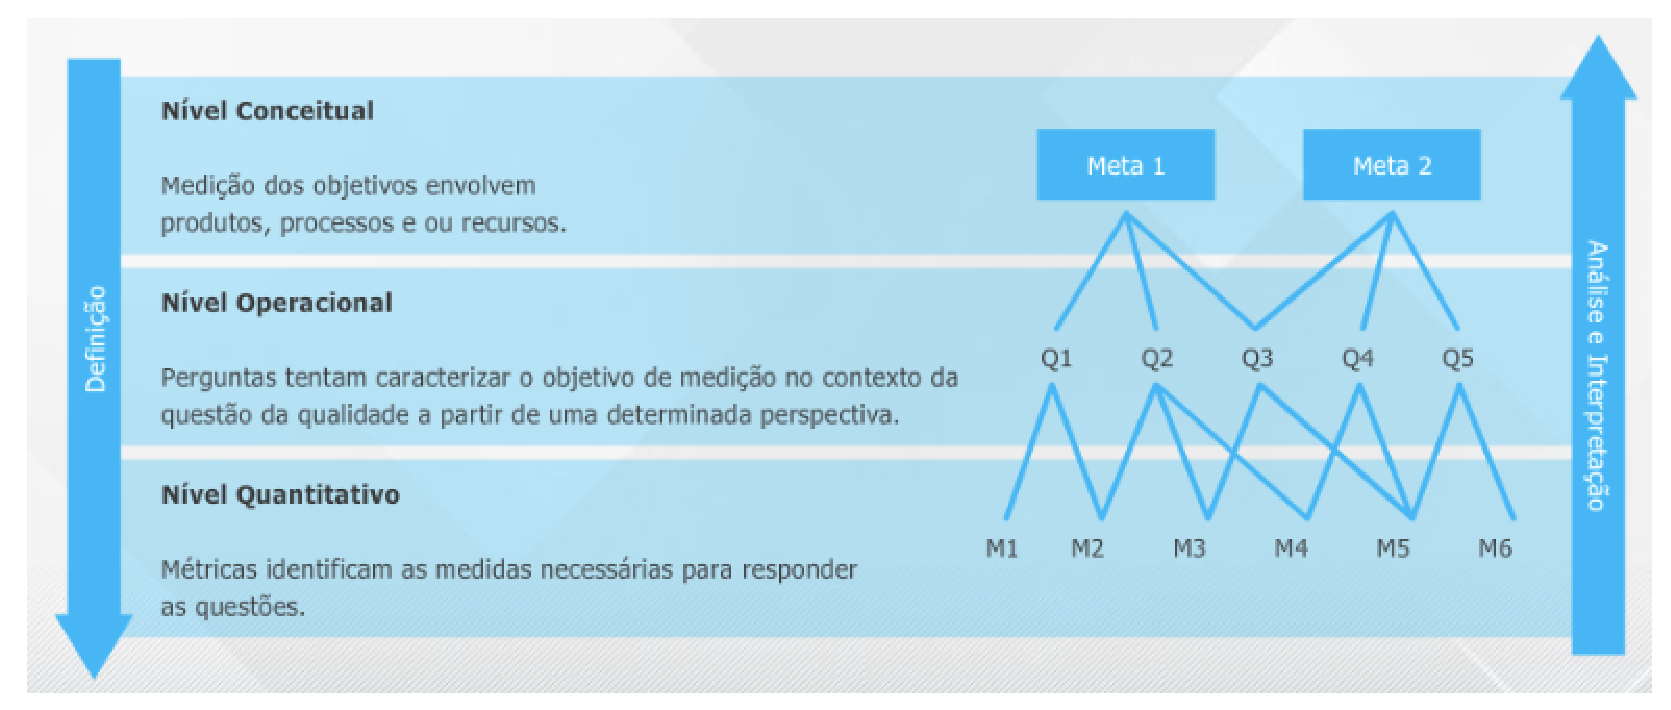
\includegraphics[keepaspectratio=true,scale=0.5]{figuras/gqm.eps}
  \caption[Níveis do GQM.]{Níveis do GQM. Fonte: \cite{junior}}
	\label{fig:gqm1}
\end{figure}

\begin{itemize}
  \item \textbf{Conceitual}: Uma meta é definida para um objetivo, envolvendo produtos, processos ou recursos.
  \item \textbf{Operacional}: Um conjunto de perguntas é elaborado com relação a cada objetivo identificado.
  \item \textbf{Quantitativo}: Um conjunto de métricas é estabelecido, de maneira a atender a cada pergunta elaborada.
\end{itemize}

\subsection{Fechamento da seção}

Um processo de medição de software direcionado aos objetivos produz medidas que provêem informações para importantes questões de negócio, previamente identificadas. Uma vez que as medidas podem ser rastreadas de volta aos objetivos da organização \cite{junior}
